\documentclass[tikz,border=2pt]{standalone}
\usepackage{amsmath}
\usetikzlibrary{arrows.meta,decorations.markings}
\begin{document}
% x' = Ax with A = [[-2,1],[0,-3]]: eigenvectors v_1 = (1,0)^T (lambda = -2) and v_2 = (1,-1)^T
% (lambda = -3); the solution from x_0 = (1,2)^T, x(t) = (3e^{-2t} - 2e^{-3t}, 2e^{-3t})^T, decays to 0
% and enters the origin along the slower direction v_1.
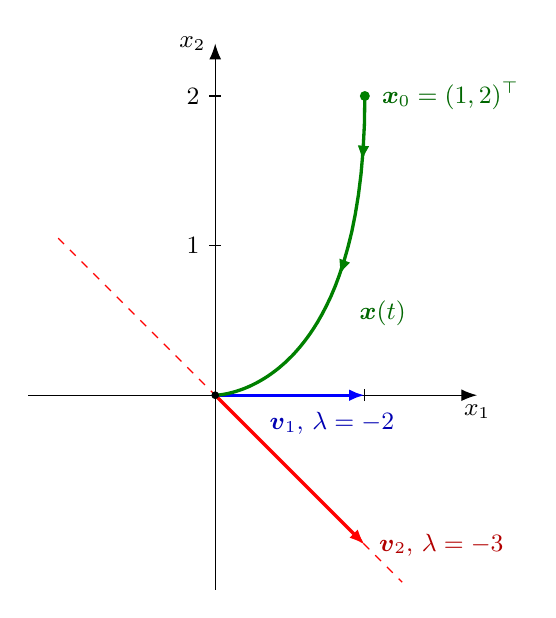
\begin{tikzpicture}[font=\small, >={Latex[length=2mm]}, x=1.9cm, y=1.9cm]
  \draw[->] (-1.25,0) -- (1.75,0) node[below] {$x_1$};
  \draw[->] (0,-1.3) -- (0,2.35) node[left] {$x_2$};
  \foreach \k in {1,2} \draw (-0.04,\k) -- (0.04,\k) node[pos=0, left] {$\k$};
  \draw (1,-0.04) -- (1,0.04);
  % eigenvector lines
  \draw[red, thin, dashed] (-1.05,1.05) -- (1.25,-1.25);
  \draw[->, red, very thick] (0,0) -- (1,-1);
  \node[red!70!black, anchor=west] at (1.03,-1.0) {$\boldsymbol{v}_2$, $\lambda=-3$};
  \draw[->, blue, very thick] (0,0) -- (1,0);
  \node[blue!70!black, anchor=north] at (0.78,-0.05) {$\boldsymbol{v}_1$, $\lambda=-2$};
  % trajectory
  \draw[green!50!black, very thick, variable=\t, domain=0:4, samples=120,
    postaction={decorate, decoration={markings,
      mark=at position 0.18 with {\arrow{>}},
      mark=at position 0.5 with {\arrow{>}}}}]
    plot ({3*exp(-2*\t)-2*exp(-3*\t)}, {2*exp(-3*\t)});
  \fill[green!50!black] (1,2) circle (1.8pt);
  \node[green!40!black, anchor=west] at (1.05,2.0) {$\boldsymbol{x}_0=(1,2)^{\top}$};
  \node[green!40!black, anchor=west] at (0.9,0.55) {$\boldsymbol{x}(t)$};
  \fill (0,0) circle (1.4pt);
\end{tikzpicture}
\end{document}
